\documentclass[a4paper,12pt]{report}

\usepackage[margin=0.75in]{geometry}
\usepackage[utf8]{inputenc}
\usepackage{t1enc}
\usepackage{lmodern}

\usepackage{xsim}
\usepackage{tasks}

\DeclareExerciseTranslation{magyar}{exercise}{feladat}
\DeclareExerciseEnvironmentTemplate{feladat}{
	{%
		\par\vspace{\baselineskip}
		\noindent
		\textbf{\GetExerciseProperty{counter}.~ \XSIMmixedcase{\GetExerciseName}}%
		\IfInsideSolutionF
		{
			\GetExercisePropertyT{subtitle}%
			{ {\normalfont\itshape\PropertyValue}}%
		}
	}
}
{}

\DeclareExerciseEnvironmentTemplate{megoldas}{
	{%
		\par\vspace{\baselineskip}
		\noindent
		\textbf{\XSIMmixedcase{\GetExerciseName}}%
		\IfInsideSolutionF
		{
			\GetExercisePropertyT{subtitle}%
			{ {\normalfont\itshape\PropertyValue}}%
		}
	}
}
{}
\xsimsetup{
	exercise/name=\XSIMtranslate{exercise},
	exercise/within=section,
	exercise/template=feladat,
	exercise/the-counter=\arabic{exercise},
	solution/name=megoldás,
	solution/print,
	solution/template=megoldas,
}

\usepackage[hungarian]{babel}
\usepackage{amsmath}
\usepackage{mathtools}
\usepackage{amsthm}
\usepackage{amsfonts}
\usepackage{amssymb}
\usepackage{graphicx}
\usepackage{wrapfig}
\graphicspath{{./images/}}
\usepackage{float}
\usepackage{multicol}

\theoremstyle{definition}
\newtheorem{definition}{Definíció}
\newtheorem*{definition*}{Definíció}
\newtheorem*{remark}{Megjegyzés}
\newtheorem{theorem}{Tétel}
\newtheorem*{theorem*}{Tétel}
\newtheorem*{example}{Példa}
\newtheorem{notation}{Jelölés}
\newtheorem*{notation*}{Jelölés}

\usepackage{tikz}
\usetikzlibrary{automata,positioning}

\title{\huge{A számításelmélet alapjai} \\[-4pt] \large gyakorlati jegyzet \vspace{-15pt}}
\author{Boda Bálint}
\date{\vspace{-12pt}2023. tavaszi félév}

\begin{document}
	\maketitle
	\vspace{-10pt}
	\tableofcontents
	\chapter{Alapfogalmak}
	\begin{definition*}[ábécé]
	Szimbólumok egy véges nemüres halmaza. Például. $ V = \left\lbrace a,b \right\rbrace $.
\end{definition*}

\begin{definition*}[szimbólum]
	Egy tetszőleges $ V $ ábécé elemeit szimbólumoknak vagy betűknek nevezzük.
\end{definition*}

\begin{definition*}[szó]
	Egy $ u \in V^* $ (V ábécé elemiből álló véges) sorozatot $ V $ feletti szónak (vagy sztringnek) nevezünk.
\end{definition*}

\section{Szavak}

\begin{definition*}
	Legyen $ u \in V^* $ egy szó, ekkor a benne lévő betűk számát $u$ hosszának nevezzük  és $ l(u) $-val vagy $\left| u \right| $-el jelöljük.
\end{definition*}

\begin{notation*}
	Egy $ \delta \in V $ betű az $ u \in V^* $ szóban lévő előfordulásinak számát $ l(u)_{\delta} $-val vagy $ \left| u \right|_{\delta} $-val jelöljük.
\end{notation*}

\begin{definition*}[üres szó]
	Legyen $V$ egy ábécé, ekkor üres szónak nevezzük azt az $ \varepsilon $ szót melyre $ \left| \varepsilon \right| = 0 $. 
\end{definition*}

\begin{remark}
	Világos, hogy $ \varepsilon \in V^* $  bármely $ V $ abécé esetén.
\end{remark}

\begin{definition*}[$ V^+ $]
	Tetszőleges $ V $ ábécé esetén $ V^+ $ jelöli az $ V $ feletti nemüres szavak halmazát, azaz a $ V^+ = V^* \setminus \left\lbrace \varepsilon \right\rbrace $ halmazt. 
\end{definition*}

\subsection{Műveletek}
\subsubsection{Konkatenáció}
\begin{definition*}
	Legyen $V$ egy ábécé és legyenek $ u = s_1 \dots s_n $ és $ v = t_1 \dots t_k $ $V$ feletti szavak. Ekkor az $uv \coloneq s_1 \dots s_n t_1 \dots t_k $ szót $u$ és $v$ konkatenáltjának nevezzük.
\end{definition*}
\paragraph{Tulajdonságok}
\begin{enumerate}
	\item{$ \left| uv \right| = \left| u \right| + \left| v \right| $}
	\item általában nem kommutatív (kivétel egyetlen betűből álló ábécék)
	\item asszociatív: $ u,v,w \in V^* \implies u(vw) = (uv)w $
	\item $ \forall u,v \in V^*: uv \in V^* $ ($ V^* $ a konkatenáció műveletére zárt)
	\item létezik egységelem: $ \forall u \in V^*: u\varepsilon = u $
\end{enumerate}
Így $V^*$ félcsoport.

\newpage
\subsubsection{Hatványozás}
\begin{definition*}
	Legyen $ i \in \mathbb{N}^+ $ és $ u \in V^* $. Ekkor $u$ $i$-edik hatványának nevezzük az $u$ szó $i$ darab példányának konkatenáltját.
	\[
	u^0 = \varepsilon, \; u^i = uu^{i-1} \, (i \in \mathbb{N}^+)
	\]
\end{definition*}

\begin{remark}
	Nyilván $\varepsilon^0 = \varepsilon$.
\end{remark}
\paragraph{Tulajdonságok}
\begin{enumerate}
	\item{$u^{n+k} = u^n u^k \; \left( k,n \in \mathbb{N} \right)  $}
	\item{$ (ab)^n \ne a^nb^n $}
\end{enumerate}

\subsubsection{Tükörkép}
\begin{definition*}
	Legyen $ u = a_1 \dots a_n $, ekkor a szó tükörképének (megfordítottjának) nevezzük a
	\[
	u^R = a_n \dots a_1 \; (1 \le i \le n: u_i = u^R_{n+1-i})
	\]
	szót. Alternatív jelölés: $u^{-1}$, rev($ u $).
\end{definition*}
\begin{remark}
	Ha $u = u^R$ a szót palindrómának (vagy palindrom tulajdonságúnak) nevezzük.
\end{remark}

\paragraph{Tulajdonságok}\mbox{}\\[-20pt]

\begin{multicols}{2}
	\begin{enumerate}
		\item{$ \varepsilon^R = \varepsilon $}
		\item{$ \left(u^R \right)^R = u $}
		\item{$ \left( uv \right)^R = v^R u^R $}
		\item{$ \left( u^i \right)^R = \left( u^R \right)^i \; (i \in \mathbb{N}) $}
	\end{enumerate}
\end{multicols}
\subsection{Résszavak}
\subsection{Résszó}
Legyen $V$ egy ábécé és legyenek $u$ és $v$ szavak $V$ felett.
\begin{definition*}[résszó]
	Az $u$ szó résszava a $v$ szónak, ha $ \exists x,y \in V^*: v = xuy $.
\end{definition*}
\begin{definition*}[valódi résszó]
	Az $u$ szó valód résszava a $v$ szónak, ha résszó és $ u \ne v $ és $ u \ne \varepsilon $.
\end{definition*}
\begin{definition*}[prefixum]
	Ha, $ v = xuy$, úgy hogy $x = \varepsilon$, akkor $u$-t $v$ prefixumának nevezzük.
\end{definition*}
\begin{definition*}[szuffixum]
	Ha, $ v = xuy$, úgy hogy $y = \varepsilon$, akkor $u$-t $v$ szuffixumának nevezzük.
\end{definition*}
\noindent
Az $u$ szót $v$ valódi prefixumainak/szuffixumainak nevezzük, ha $u \ne \varepsilon \land u \ne v $.

\section{Nyelv}
\begin{definition*}[nyelv]
	Legyen $V$ egy ábécé, ekkor nyelvnek nevezzük az $ L \subseteq V^* $ halmazt. Ekkor $L$-t $V$
\end{definition*}

\begin{notation*}
	$ \emptyset $-el jelöljük az üres nyelvet. $\emptyset \ne \left\lbrace \varepsilon \right\rbrace $ 
\end{notation*}

\subsection{Műveletek}
\noindent
Mivel a nyelvek halmazok értelmezzük az unió, metszet, különbség és komplementer műveleteket. 
\subsubsection{Konkatenáció}

\begin{definition*}
	Legyen $V^*$ egy ábécé és $L_1, L_2 \subseteq V^*$, ekkor $L_1$ és $L_2$ konkatenációjának nevezzük az 
	\[
	L_1L_2 = \left\lbrace u_1,u_2 | u_1 \in L_1, u_2 \in L_2 \right\rbrace 
	\]
	a nyelvet.
\end{definition*}
\begin{example}
	\[
	\left\lbrace a,b \right\rbrace \left\lbrace ab,b \right\rbrace = \left\lbrace aab, ab, bab, bb \right\rbrace   
	\]
\end{example}
\paragraph{Tulajdonságok}
\begin{enumerate}
	\item Minden $ L $ nyelv esetén: $ \left\lbrace \varepsilon \right\rbrace L = L \left\lbrace \varepsilon \right\rbrace $
	\item Asszociatív
	\item Egységelem: $ \left\lbrace \varepsilon \right\rbrace $.
\end{enumerate}

\subsubsection{Hatványozás}
\begin{definition*}
	Legyen $V^*$ egy ábécé és $L \subseteq V^* $, ekkor $L$ $i$-edik hatványának nevezzük a
	\[
	L^0 = \left\lbrace \varepsilon \right\rbrace, \qquad L^i = LL^{i-1} \quad (i \ge 1)
	\]
	a nyelvet.
\end{definition*}
\begin{remark}
	$ \emptyset^0 = \left\lbrace \varepsilon \right\rbrace $. 
\end{remark}
\subsubsection{Iteratív lezárt}
\begin{definition*}
	Egy $L$ nyelv iteratív lezártjának nevezzük az
	\[
	L^* = \bigcup_{i \ge 0}{L^i}=L^0 \cup L^1 \cup \dots
	\]
	nyelvet.
\end{definition*}

\subsubsection{Pozitív lezárt}
\begin{definition*}
	Egy $L$ nyelv pozitív lezártjának nevezzük az
	\[
	L^+ = \bigcup_{i \ge 1}{L^i}=L^0 \cup L^1 \cup \dots = L^* \setminus \left\lbrace \varepsilon \right\rbrace 
	\]
	nyelvet.
\end{definition*}
\newpage
\subsection{Feladatok}
\subsubsection{}
Legyenek
\begin{align*}
	L_1 &= \left\lbrace a, bb, aba \right\rbrace \\
	L_2 &= \left\lbrace ab^n \; | \; n \ge 0 \right\rbrace = \left\lbrace a, ab, abb, \dots \right\rbrace  \\
	L_3 &= \left\lbrace u \in \left\lbrace a,b \right\rbrace ^* \; | \; l_a(u) = l_b(u) \right\rbrace
	= \left\lbrace \varepsilon, ab, ba, \dots \right\rbrace  \\
	L_4 &= \left\lbrace u \in \left\lbrace a,b \right\rbrace ^* \; | \; l_b(u) \bmod 2  = 0 \right\rbrace
	= \left\lbrace \varepsilon, a, bb, abb, aabb, \dots \right\rbrace \\
	L_5 &= \left\lbrace \varepsilon, ba \right\rbrace
\end{align*}
nyelvek. Határozzuk meg:
\begin{align*}
	L_1 \cap L_2 &= \left\lbrace a \right\rbrace \\
	L_1 \cap L_3 &= \emptyset \\
	L_1 \cap L_4 &= \left\lbrace a, bb \right\rbrace \\
	L_2 \setminus L_1 &= \left\lbrace ab^n \; | \; n \ge 1 \right\rbrace \\
	L_1L_5 &= \left\lbrace a, aba, bb, bbba, ababa \right\rbrace \\
	L_1^2 &= \left\lbrace aa, abb, aaba, bba, bbbb, bbaba, abaa, ababb, abaaba \right\rbrace 
\end{align*}
Legyenek
\begin{align*}
	L_1 &= \left\lbrace a^nb^m \; | \; m \ge n \land n \ge 0 \right\rbrace = \left\lbrace \varepsilon, b, ab, abb, \dots \right\rbrace  \\
	L_2 &= \left\lbrace ab \right\rbrace^* = \left\lbrace \varepsilon, ab, abab, \dots \right\rbrace 
\end{align*}
nyelvek. Határozzuk meg:
\begin{align*}
	L_1 \cap L_2 &= \left\lbrace \varepsilon, ab \right\rbrace \\
	L_1 \setminus L_2^* &= \left\lbrace a^nb^m \; | \; m \ge n \ge 2 \right\rbrace \cup \left\lbrace b \right\rbrace^+ \cup \left\lbrace ab^n \; | \; n \ge 1 \right\rbrace \\
	L_1^* &= \left\lbrace \varepsilon, b, ab, abb, bb, bab, abab, \dots \right\rbrace \\
	L_2 \ L_1^* &= \emptyset \qquad (ab \in L_1^* \text{ miatt}) \\
	L_2^* &= L_2
\end{align*}
	\chapter{Generatív grammatika}
	\section{Generatív grammatika}
\begin{definition*}[grammatika]
	Egy $ G = (N, T, P, S) $ rendezett négyest (generatív) grammatikának vagy nyelvtannak nevezünk, ha $N$ és $T$ diszjunkt (azaz $N \cap T = \emptyset $) véges ábécék. Ekkor 
	\begin{itemize}
		\item $N$ a nem terminális szimbólumok halmaza,
		\item $T$ (vagy $ \Sigma $) a terminális szimbólumok halmaza,
		\item $S \in N$ a grammatika kezdőszimbóluma,
		\item $P = \left\lbrace (x,y) \; | \; x,y \in \left( N \cup T \right)^*  \text{ szavak úgy, hogy } x \text{ legalább egy nem terminális betűt tartalmaz} \right\rbrace $, az ún. (átírási) szabályok (vagy produkciók) halmaza.
	\end{itemize}
\end{definition*}

\begin{notation*}
	Gyakran $(x,y)$ helyett az $x \rightarrow y$ jelölést használjuk, egy szabály leírására. Természetesen ez csak akkor lehetséges ha az adott ábécének nem eleme $\rightarrow$. 
\end{notation*}
\vspace{6pt}
\begin{definition*}[egylépéses levezetés]
	Legyen $ G = (N, T, P, S) $ egy grammatika és legyen $u, v \in (N \cup T)^*$. Azt mondjuk $v$ közvetlen levezethető az $u$ szóból $G$-ben (jelekkel: $ u \Rightarrow_G v $), ha
	\[
	\exists (x, y) \in P: \; u = u_1xu_2 \text{ és } v = u_1yu_2, \quad \left(u_1, u_2 \in (N \cup T)^*\right)
	\]  
\end{definition*}
\vspace{6pt}
\begin{definition*}[többlépéses levezetés]
	Legyen $ G = (N, T, P, S) $ egy grammatika és legyen $u, v \in (N \cup T)^*$. Azt mondjuk $v$ több lépésben levezethető az $u$ szóból $G$-ben (jelekkel: $ u \Rightarrow_G^* v $), ha
	\[
	u = v \lor \exists \left( n \ge 1 \land w_0,\dots,w_n \in (N \cup T)^* \right)  \text{, hogy } w_{i-1} \Rightarrow_G w_i \, (1 \le i \le n), \; w_0 = u \text{ és } w_n = v
	\]
\end{definition*}
\vspace{6pt}
\begin{definition*}[generált nyelv]
	Legyen $ G = (N, T, P, S) $ egy grammatika, ekkor a $G$ által generált nyelvnek nevezzük az $S$ kezdőszimbólumból több lépésben levezethető terminális szavak halmazát, azaz a
	\[
		L(G) = \left\lbrace u \in T^* \; | \; S \Rightarrow_G^* u \right\rbrace 
	\]
	nyelvet.
\end{definition*}

\begin{example}
	Legyen
	\begin{align*}
		G &= \left( \left\lbrace S, A, B \right\rbrace, \left\lbrace a,b \right\rbrace P, S \right) \\
		P &= \left\lbrace S \rightarrow B | bb, \; B \rightarrow aaA, \; A \rightarrow a | \varepsilon \ \right\rbrace 
	\end{align*}
	Adjuk meg $L(G)$-t!

	\begin{remark}
		Egy $ S \rightarrow B | bb $ az $ S \rightarrow B $ és $ S \rightarrow bb $ szabályokat jelöli.
	\end{remark}

	\begin{align*}
		S &\rightarrow bb \\
		S &\rightarrow B \rightarrow aaA \rightarrow a \\
		S &\rightarrow B \rightarrow aaA \rightarrow \varepsilon
	\end{align*}
	Így: $L(G) = \left\lbrace bb, aa, a \right\rbrace $. 
\end{example}

\subsection{Feladatok}

\begin{exercise}
	Legyen $ G_i = (\left\lbrace S, A, B \right\rbrace, \left\lbrace a,b \right\rbrace, P_i, S) $. Határozzuk meg az $L(G_i)$ nyelvet, ha
	\begin{itemize}
		\item $P_1 = \left\lbrace S \rightarrow aaS | a \right\rbrace $
		\item $P_2 = \left\lbrace S \rightarrow aSb | \varepsilon \right\rbrace $
		\item $P_3 = \left\lbrace S \rightarrow ASB | \varepsilon, \, AB \rightarrow BA, \, BA \rightarrow AB, \, A \rightarrow a, \, B \rightarrow b \right\rbrace $
	\end{itemize}
\end{exercise}
		
\begin{solution}
	\begin{align*}
		L(G_1) &= \left\lbrace a, aaa, aaaaa \dots \right\rbrace = \left\lbrace a^{(2n+1)} \; | \; n \ge 0 \right\rbrace \\
		L(G_2) &= \left\lbrace \varepsilon, ab, aabb \dots \right\rbrace = \left\lbrace a^nb^n \; | \; n \ge 0 \right\rbrace
	\end{align*}
	A harmadik nyelv meghatározása már nehezebb feladat. Tekintsünk pár példa levezetést:
	\begin{align*}
		S &\rightarrow A\underline{S}B \rightarrow \underline{A}B \rightarrow a\underline{B} \rightarrow ab \\
		S &\rightarrow ASB \rightarrow AB \rightarrow BA \rightarrow bA \rightarrow ba \\
		S &\rightarrow A\underline{S}B \rightarrow AA\underline{S}BB \rightarrow A\underline{AB}B \rightarrow \underline{AB}AB \rightarrow BA\underline{AB} \rightarrow \underline{B}ABA \rightarrow \dots \rightarrow baba \\
		S &\rightarrow ASB \rightarrow AASBB \rightarrow AABB \rightarrow ABAB \rightarrow BAAB \rightarrow baab
	\end{align*}
	Ezek alapján $L(G_3) = \left\lbrace u \in \left\lbrace a,b \right\rbrace^* \; | \; l_a(u) = l_b(u) \right\rbrace $.
\end{solution}

\section{A grammatikák Chomsky féle osztályzása}
Legyen $ G = (N, T, P, S) $ egy grammatika. A $G$ grammatika $i$-típusú $ (i = 0,1,2,3) $, ha a $P$ szabályhalmazra teljesülnek a következők:
\begin{itemize}
	\item $ i = 0 $ (mondatszerkezetű grammatika): nincs korlátozás
	\item { $ i = 1 $ (környezetfüggő grammatika):
		\begin{itemize}
			\item $P$ minden szabálya $u_1Au_2 \rightarrow u_1vu_2 $ alakú, ahol $u_1, u_2, v \in (N \cup T)^*, A \in N $ és $ v \ne \varepsilon $
			\item Kivétel: $P$ tartalmazhatja az $ S \rightarrow \varepsilon $ szabályt, de csak akkor, ha $S$ nem fordul elő egyetlen szabály jobb oldalán sem.
		\end{itemize}
	}
	\item { $ i = 2 $ (környezetfüggetlen): $ P $ minden szabálya $A \rightarrow v $ alakú ($A \in N, \; v \in (N \cup T)^*) $
	}
	\item { $ i = 3 $ (reguláris): $ P $ minden szabálya $A \rightarrow uB $ vagy $A \rightarrow u $ alakú ($A,B \in N, \; u \in T^*) $
	}
\end{itemize}
Az adott osztályokat $\mathcal{G}_i$-vel jelöljük.

\begin{definition*}[nyelvosztály]
	Az $i$ típusú nyelvek osztályának nevezzük a 
	\[
	\mathcal{L}_i = \left\lbrace L \; | \; \exists G \in \mathcal{G}_i \text{, hogy } L = L(G) \right\rbrace 
	\]
\end{definition*}

\begin{theorem}[Chomsky nyelvhierarchia tétel]
	\[
		\mathcal{L}_3 \subset \mathcal{L}_2 \subset \mathcal{L}_1 \subset \mathcal{L}_0
	\]
\end{theorem}

\subsection{Feladatok}
\setcounter{exercise}{0}
\begin{exercise}
	Írjuk fel azt a grammatikát, mely a 4-el osztható bináris számok nyelvét generálja! Milyen osztályba sorolható a generált nyelv?
\end{exercise}

\begin{solution}
	Egy kettes számrendszerbeli szám akkor osztható néggyel, ha utolsó két számjegye 0. Gondoskodnunk kell továbbá arról, hogy ne legyenek felesleges nullák az elején. Így
	\[
	G = \left( \left\lbrace S, B \right\rbrace, \, \left\lbrace 0,1, \varepsilon \right\rbrace, \, \left\lbrace  S \rightarrow \underbrace{0}_{3.} | \underbrace{1B00}_{2.}, \,  B \rightarrow \underbrace{\varepsilon}_3.|\underbrace{0B}_{3.}|\underbrace{1B}_{3.} \right\rbrace , \, S \right)
	\]
	(Az adott szabály jobb oldala alatt tüntettem fel annak szintjét.) Mivel kettes a legkisebb szint ezért a generált nyelv is 2-es szintű.
	\\[4pt]
	A feladat megoldható más módon is:
	\[
	G = \left( \left\lbrace S, A \right\rbrace, \, \left\lbrace 0,1, \varepsilon \right\rbrace, \, \left\lbrace  S \rightarrow 0 | 1A, \,  A \rightarrow \varepsilon|0A|1A \right\rbrace , \, S \right)
	\]
	amiből már reguláris nyelv adódik.
\end{solution}

\begin{exercise}
	Írjuk fel azt a grammatikát, ami az $ L(G) = \left\lbrace a^n b^m c^n \; | n \ge 0, \, m \ge 3 \right\rbrace  $, nyelvet generálja!
\end{exercise}
\begin{solution}
	Írjuk fel $L(G)$ néhány elemét: $ \left\lbrace bbb, abbbc, aabbbcc \dots \right\rbrace $. Így $ G = (\left\lbrace  S,A,B,C \right\rbrace , \left\lbrace a,b,c \right\rbrace, P, S) $, ahol
	\begin{align*}
		P = \left\lbrace \begin{array}{l}
			S \rightarrow ASC, \\
			S \rightarrow BBB, \\
			A \rightarrow a, \\
			B \rightarrow b, \\
			C \rightarrow c
		\end{array} \right\rbrace 
	\end{align*}
\end{solution}

\section{Reguláris kifejezések}
	\chapter{Véges automaták}
	Véges automatának nevezünk egy olyan analitikus eszközt, mely képes eldönteni egy adott szóról, hogy az általa ismert reguláris nyelv eleme-e.

\section{Alapfogalmak}
\begin{definition*}
	\textbf{Determinisztikus véges automatának} (DVA) nevezünk egy $ A = \left( Q, \Sigma, \delta, Q_0, F \right) $ rendezett ötöst, ahol
	\begin{itemize}
		\item $ Q $ a lehetséges állapotok véges nemüres halmaza
		\item $ \Sigma $ az inputszimbólumok ábécéje
		\item $ \delta: Q \times \Sigma \rightarrow Q $ az ún. állapotátmeneti függvény
		\item $ q_0 \in Q $ a kezdőállapot
		\item $ F \subseteq Q $ az elfogadó állapotok halmaza.
	\end{itemize}
\end{definition*}

\noindent
Legyen $ A = \left( \left\lbrace q_0, q_1, q_2 \right\rbrace , \left\lbrace a,b \right\rbrace , \delta, q_0, \left\lbrace q_2 \right\rbrace \right) $
$ \delta $ több módon is megadható:
\begin{itemize}
	\item{
		Függvény: $ \delta{\left( q_0, a \right) } = q_1, \; \delta{\left( q_0, b \right) } = q_2, \; \delta{\left( q_1, a \right) } = q_0 $
	}
	\item{
		Grammatikaszerűen: $ M_\delta = \left\lbrace q_0 a \rightarrow q_1, \; q_0 b \rightarrow q_2, \; q_1a \rightarrow q_0 \right\rbrace $
	}
	\item{
		Táblázatosan:
		\begin{table}[H]
			\centering
			\begin{tabular}{|c|c|c|}
				\hline
				$ $ & $ a $ & $ b $ \\
				\hline
				$ \rightarrow q_0 $ & $ q_1 $  & $ q_2 $  \\
				\hline
				$ q_1 $ & $ q_0 $  & $ - $  \\
				\hline
				$ \leftarrow q_2 $ & $ - $  & $ - $  \\
				\hline
			\end{tabular}
		\end{table}
		A kezdőállapotot $ \rightarrow $-val, az elfogadó állapotokat $ \leftarrow $-val jelöljük.
	}
	\item{
		Állapotátmeneti gráffal:
		
		\begin{figure}[H]
			\centering
			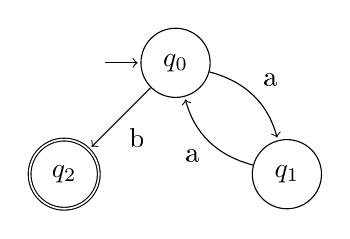
\begin{tikzpicture}[shorten >=1pt,node distance=2cm,on grid,auto] 
				\node[state,initial, initial text=] (q_0)   {$q_0$}; 
				\node[state] (q_1) [below right=of q_0] {$q_1$}; 
				\node[state, accepting] (q_2) [below left=of q_0] {$q_2$}; 
				\path[->] 
				(q_0) edge [bend left] node {a} (q_1)
				(q_1) edge [bend left] node {a} (q_0)
				(q_0) edge node {b} (q_2);
			\end{tikzpicture}
		\end{figure}
		
		ahol, $ \rightarrow $ jelöli a kezdőállapotot és dupla kör az elfogadó állapotokat.
	}
\end{itemize}
\newpage
\begin{definition*}
	\textbf{Nemdeterminisztikus véges automatát} hasonlóan definiáljuk, annyi különbséggel, hogy a $ \delta $  függvény $ Q $ helyett, $ Q $ hatványhalmazába  képez, azaz $ \delta: Q \times \Sigma \rightarrow \mathcal{P}{\left( Q \right) } $.
\end{definition*}
\noindent
$ \delta $ hasonlóan adható meg mint DVA esetén, és a nemdeterminisztikusság minden esetben könnyen leolvasható:
\begin{itemize}
	\item függvény értéke halmaz lesz
	\item grammatika szerű jelölésben vagy ($ | $) jelenik meg valamelyik kifejezés jobb oldalán
	\item táblázatban halmazok vannak
	\item egy csúcsból több azonos címkéjű él vezet ki
\end{itemize}

\begin{definition*}[konfiguráció]
	Legyen $ A = \left( Q, \Sigma, \delta, Q_0, F \right) $ egy véges automata, ekkor \textbf{konfigurációnak} nevezünk egy $ u \in Q\Sigma^* $ szót.
\end{definition*}

\begin{definition*}[egylépéses redukció]
	Legyen $ A = \left( Q, \Sigma, \delta, Q_0, F \right) $ egy véges automata és legyenek $u, v$ konfigurációk. Azt mondjuk $u$ egy lépésben \text{redukálható} $v$-re, ha létezik $ p \in \delta(q, a) $ szabály és $ w \in \Sigma^* $ szó, hogy $ u = qaw $ és $ v = pw $.
\end{definition*}

\begin{definition*}[redukció]
	Az $ A = \left( Q, \Sigma, \delta, Q_0, F \right) $ véges automata az $ u \in Q\Sigma^* $ szót a
	$ v \in Q\Sigma^* $ szóra redukálja (jelölés: $ u \Rightarrow_A^* v $), ha vagy $ u = v $ vagy
	valamely $ k \ge 1 $-re léteznek $w_0, \dots , w_k $ konfigurációk melyekre
	$ w_{i-1} \Rightarrow_A w_i (1 \ge i \ge k ) $, $ w_0 = u $ és $ w_k = v $.
\end{definition*}

\begin{definition*}[felismert nyelv]
	Legyen $ A = \left( Q, \Sigma, \delta, Q_0, F \right) $ egy véges automata. Az $A$ automata által elfogadott (vagy felismert) nyelvnek nevezzük az
	\[
	L(A) = \left\lbrace u \in \Sigma^* | q_0u \Rightarrow_A^*p \, \land \, q_0 \in Q \, \land \, p \in F \right\rbrace 
	\]
	nyelvet. 
\end{definition*}
\newpage
\subsection{Feladatok}
\begin{exercise}
	Adjunk meg automatát és generatív grammatikát a következő reguláris kifejezésekhez:
	\begin{tasks}
		\task $ \left(a+b\right)^*a $
		\task $ 1\left(1+0\right)^*0+0 $
		\task $ a\left(a+b+c\left(a+b\right)\right)^* $
	\end{tasks}
\end{exercise}
\begin{solution}[print]
	\begin{tasks}
		\task{
			Grammatika: $ \left( \left\lbrace S \right\rbrace, \, \left\lbrace a,b \right\rbrace, \, \left\lbrace S \rightarrow aS \mid bS \mid a \right\rbrace  \right) $
			\\[8pt]
			Automata:
			\begin{figure}[H]
				\centering
				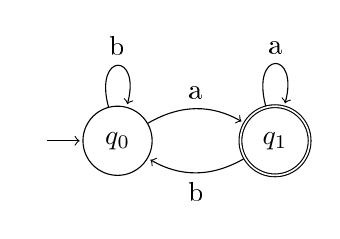
\begin{tikzpicture}[shorten >=1pt,node distance=2cm,on grid,auto] 
					\node[state,initial, initial text=] (q_0)   {$q_0$}; 
					\node[state, accepting] (q_1) [right=of q_0] {$q_1$}; 
					\path[->] 
					(q_0) edge [loop above] node {b}
					(q_0) edge [bend left] node {a} (q_1)
					(q_1) edge [loop above] node {a}
					(q_1) edge [bend left] node {b} (q_0);
				\end{tikzpicture}
			\end{figure}
		}
		\task{
			Grammatika: $ \left( \left\lbrace S, C \right\rbrace, \, \left\lbrace 0,1 \right\rbrace, \, P, \, S  \right) $, ahol \\
			$ P = \left\lbrace S \rightarrow 0 \mid 1C, \, C \rightarrow 0C \mid 1C \mid 0 \right\rbrace $
			\\[8pt]
			Automata:
			\begin{figure}[H]
				\centering
				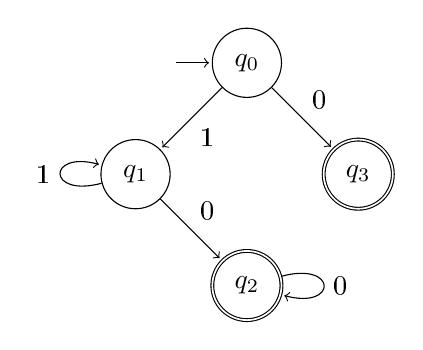
\begin{tikzpicture}[shorten >=1pt,node distance=2cm,on grid,auto] 
					\node[state,initial, initial text=] (q_0)   {$q_0$}; 
					\node[state] (q_1) [below left=of q_0] {$q_1$};
					\node[state, accepting] (q_2) [below right=of q_1] {$q_2$};
					\node[state, accepting] (q_3) [below right=of q_0] {$q_3$};
					\path[->]
					(q_0) edge node {1} (q_1)
					(q_0) edge node {0} (q_3)
					(q_1) edge [loop left] node {1} ()
					(q_1) edge node {0} (q_2)
					(q_2) edge [loop right] node {0} ()
					;
				\end{tikzpicture}
			\end{figure}
		}
		\task{
			Grammatika: $ \left( \left\lbrace S, C, E \right\rbrace, \, \left\lbrace a,b,c \right\rbrace, \, P, \, S  \right) $, ahol
			\[ P =  \left\lbrace \begin{array}{c}
				S \rightarrow aE, \\
				E \rightarrow \varepsilon \mid aE \mid bE \mid cC, \\
				C \rightarrow aE \mid bE 
			\end{array} \right\rbrace \]
			Automata:
			\begin{figure}[H]
				\centering
				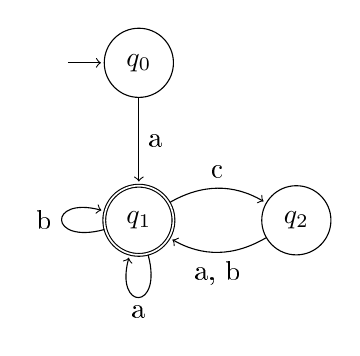
\begin{tikzpicture}[shorten >=1pt,node distance=2cm,on grid,auto] 
					\node[state,initial, initial text=] (q_0)   {$q_0$}; 
					\node[state, accepting] (q_1) [below =of q_0] {$q_1$};
					\node[state] (q_2) [right=of q_1] {$q_2$};
					\path[->]
					(q_0) edge node {a} (q_1)
					(q_1) edge [loop below] node {a} ()
					(q_1) edge [loop left] node {b} ()
					(q_1) edge [bend left] node {c} (q_2)
					(q_2) edge [bend left] node {a, b} (q_1)
					;
				\end{tikzpicture}
			\end{figure}
		}
	\end{tasks}
\end{solution}

\begin{exercise}
	Adjunk meg automatát, mely felismeri a következő nyelveket:
	\begin{tasks}
		\task 3-al osztható természetes számok (vezető nullákat nem kezelve)
		\task 3-al osztható egész számok (vezető nullákat kezelve)
	\end{tasks}
\end{exercise}
\begin{solution}
	\begin{tasks}
		\task{
			Egy szám akkor osztható hárommal, ha számjegyeinek összege osztható hárommal. Az automata azonban nem képes sem aritmetikai műveletekre, sem ezek eredményének eltárolására. Megfeleltethetjük, azonban a különböző állapotokat a hárommal való osztás maradékosztályainak.
			
			Például: Legyen a vizsgálandó szó 156. Az automata először feldolgozza az 1-es szimbólumot, melynek hatására a $ q_1 $ állapotba kerül, mivel $1 \mod 3 = 1$. Ezt követően, mivel jelenleg a $ q_1$ állapotban vagyunk és $5 \mod 3 = 2$, ezért a 0-ás maradékosztályba azaz $q_0$-ba kerülünk.Ezután mivel $ 6 \mod 3 = 0 $, ezért a $ q_0$ állapotban maradunk.
			
			\begin{figure}[H]
				\centering
				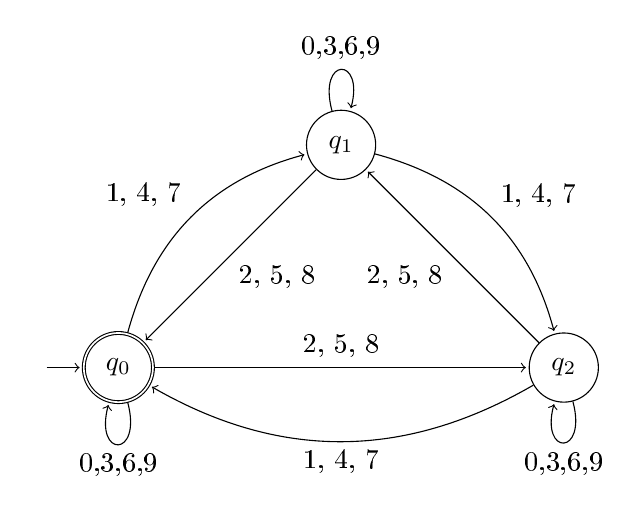
\begin{tikzpicture}[shorten >=1pt,node distance=4cm,on grid,auto] 
					\node[state,initial, initial text=, accepting] (q_0)   {$q_0$}; 
					\node[state] (q_1) [above right =of q_0] {$q_1$};
					\node[state] (q_2) [below right=of q_1] {$q_2$};
					\path[->]
					(q_0) edge [loop below] node {0,3,6,9} ()
					(q_0) edge [bend left] node {1, 4, 7} (q_1)
					(q_1) edge node {2, 5, 8} (q_0)
					(q_1) edge [loop above] node {0,3,6,9} ()
					(q_1) edge [bend left] node {1, 4, 7} (q_2)
					(q_2) edge node {2, 5, 8} (q_1)
					(q_2) edge [loop below] node {0,3,6,9} ()
					(q_2) edge [bend left] node {1, 4, 7} (q_0)
					(q_0) edge node {2, 5, 8} (q_2)
					;
				\end{tikzpicture}
			\end{figure}
		}
		\task{
			A megoldás nagyon hasonló annyi különbséggel, hogy fel kell vennünk két extra állapotot. Az egyik állapot a mínusz jelet a másik pedig a vezető nullákat fogja kezelni.
			
			\begin{figure}[H]
				\centering
				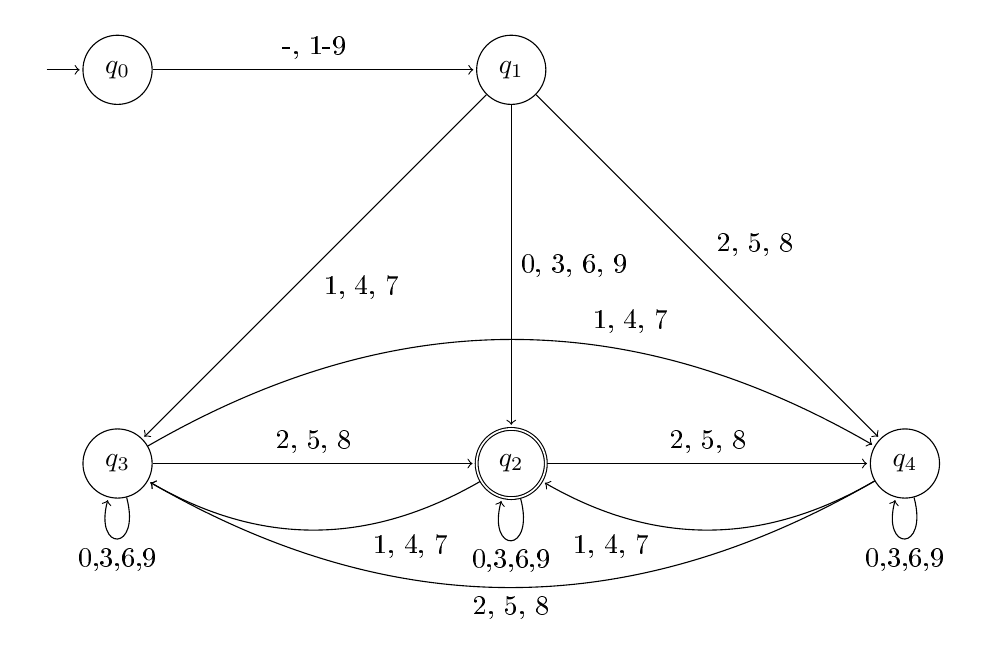
\begin{tikzpicture}[shorten >=1pt,node distance=5cm,on grid,auto]
					\node[state,initial, initial text=] (q_0)   {$q_0$};
					\node[state] (q_1) [right =of q_0] {$q_1$};
					\node[state, accepting] (q_2) [below=of q_1] {$q_2$};
					\node[state] (q_3) [left =of q_2] {$q_3$};
					\node[state] (q_4) [right =of q_2] {$q_4$};
					\path[->]
					(q_0) edge node {-, 1-9} (q_1)
					(q_1) edge node {0, 3, 6, 9} (q_2)
					(q_1) edge node {1, 4, 7} (q_3)
					(q_1) edge node {2, 5, 8} (q_4)
					(q_2) edge [loop below] node {0,3,6,9} ()
					(q_2) edge [bend left, pos=0.35] node {1, 4, 7} (q_3)
					(q_3) edge node {2, 5, 8} (q_2)
					(q_3) edge [loop below] node {0,3,6,9} ()
					(q_3) edge [bend left, pos = 0.6] node {1, 4, 7} (q_4)
					(q_4) edge [bend left] node {2, 5, 8} (q_3)
					(q_4) edge [loop below] node {0,3,6,9} ()
					(q_4) edge [bend left, pos=0.65] node {1, 4, 7} (q_2)
					(q_2) edge node {2, 5, 8} (q_4)
					;
				\end{tikzpicture}
			\end{figure}
		}
	\end{tasks}
\end{solution}
	\section{Automaták determinizálása}
Alapötlet: hozzunk létre összevont állapotokat pl. az $ \left\lbrace q_1, q_2, q_3 \right\rbrace $ állapotot vonjuk össze a $ q_{123} $ állapottá. 
\begin{example}
	Tekintsük a következő automatát:
	
	\begin{multicols}{2}
		\begin{figure}[H]
			\centering
			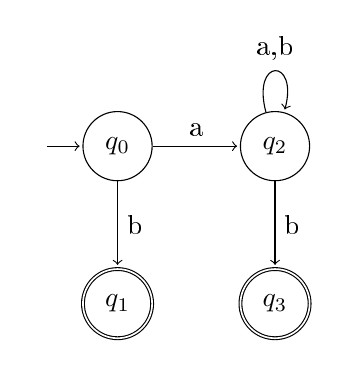
\begin{tikzpicture}[shorten >=1pt,node distance=2cm,on grid,auto] 
				\node[state,initial,initial text=] (q_0)   {$q_0$}; 
				\node[state, accepting] (q_1) [below =of q_0] {$q_1$}; 
				\node[state] (q_2) [right=of q_0] {$q_2$}; 
				\node[state,accepting](q_3) [below=of q_2] {$q_3$};
				\path[->] 
				(q_0) edge  node {b} (q_1)
				edge  node {a} (q_2)
				(q_2) edge [loop above] node {a,b} ()
				(q_2) edge  node {b} (q_3) ;
			\end{tikzpicture}
		\end{figure}
		\begin{table}[H]
			\centering
			$$
			\begin{array}{|c|c|c|}
				\hline
				& a & b \\
				\hline
				\rightarrow q_0 & \left\lbrace q_2 \right\rbrace & \left\lbrace q_1 \right\rbrace \\
				\hline
				q_1 & \varnothing  &  \varnothing \\
				\hline
				\leftarrow q_2 & \left\lbrace q_2 \right\rbrace & \left\lbrace q_2, q_3 \right\rbrace   \\
				\hline
				\leftarrow q_3 & \varnothing  & \varnothing \\
				\hline
			\end{array}
			$$
		\end{table}
	\end{multicols}
	\begin{remark}
		A nemdeterminisztikus automaták esetében a táblázatban gyakran egyelemű állapothalmazok helyett csak magát az állapotot írjuk le.
	\end{remark}
	\noindent
	Világos hogy az automata nem determinisztikus, ezért determinizáljuk: Az $q_0$ és $q_1$ sorokat változatlanul leírjuk a $q_2$ sorban azonban el kell végeznünk a $q_2$ és a $q_3$ összevonását.
	\begin{table}[H]
		\centering
		$$
		\begin{array}{|c|c|c|}
			\hline
			& a & b \\
			\hline
			\rightarrow q_0 &  q_2 & q_1 \\
			\hline
			q_1 & \varnothing  &  \varnothing \\
			\hline
			\leftarrow q_2 & q_2 & q_{23}    \\
			\hline
			\leftarrow q_3 & \varnothing  & \varnothing \\
			\hline
			? q_{23}& ? & ? \\
			\hline
		\end{array}
		$$
	\end{table}
	\noindent
	Mivel $q_2$ és $q_3$ közül legalább az egyik elfogadó állapot volt így az összevont állapot is elfogadó lesz. Ezt követően már csak az összevonásokat kell elvégeznünk:
	\begin{enumerate}
		\item $ \tr{(q_{23}, a)} = \tr{(q_2, a)} \, \cup \, \tr{(q_3, a)} = \left\lbrace q_2 \right\rbrace \, \cup \, \varnothing = \left\lbrace q_2 \right\rbrace \quad \text{Egyelemű, nem kell további összevonás} $
		\item $ \tr{(q_{23}, b)} = \tr{(q_2, b)} \, \cup \, \tr{(q_3, b)} = \left\lbrace q_{23} \right\rbrace \, \cup \, \varnothing = \left\lbrace q_{23} \right\rbrace \quad \text{Egyelemű, nem kell további összevonás} $
	\end{enumerate}
	\noindent
	Így az automata:
	
	\begin{multicols}{2}
		\begin{table}[H]
			\centering
			$$
			\begin{array}{|c|c|c|}
				\hline
				& a & b \\
				\hline
				\rightarrow q_0 & q_2  & q_1 \\
				\hline
				q_1 & \varnothing  &  \varnothing \\
				\hline
				\leftarrow q_2 & q_2 & q_{23}   \\
				\hline
				\leftarrow q_3 & \varnothing  & \varnothing \\
				\hline
				\leftarrow q_{23} & q_2 & q_{23} \\
				\hline
			\end{array}
			$$
		\end{table}
		\begin{figure}[H]
			\centering
			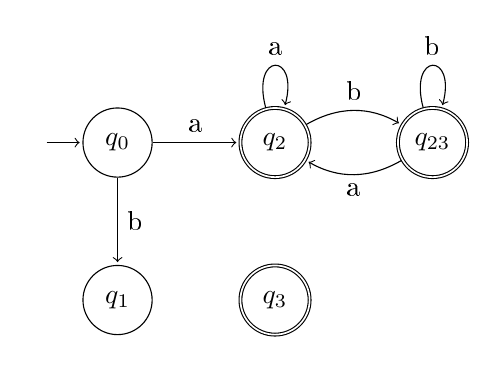
\begin{tikzpicture}[shorten >=1pt,node distance=2cm,on grid,auto] 
				\node[state,initial,initial text=] (q_0)   {$q_0$}; 
				\node[state] (q_1) [below =of q_0] {$q_1$}; 
				\node[state, accepting] (q_2) [right=of q_0] {$q_2$}; 
				\node[state,accepting](q_3) [below=of q_2] {$q_3$};
				\node[state,accepting](q_23) [right=of q_2] {$q_{23}$};
				\path[->] 
				(q_0) edge  node {b} (q_1)
				edge  node {a} (q_2)
				(q_2) edge [loop above] node {a} ()
				(q_2) edge [bend left] node {b} (q_23)
				(q_23) edge [bend left]  node {a} (q_2)
				(q_23) edge [loop above] node {b} ();
			\end{tikzpicture}
		\end{figure}
	\end{multicols}
	Észrevehetjük, hogy a $q_3$ állapot elérhetetlenné vált, azaz az automata elvesztette összefüggőségét. Az összefüggőség megőrzéséhez bevezethetünk egy egyszerű változtatást az algoritmusba, hogy egy sort állapotot csak akkor veszünk az új automatához, ha arra egy korábbi sor már hivatkozik.
\end{example}
\newpage
\noindent
Tekintsünk egy bonyolultabb példát:
\begin{example}
	Determinizáljuk a következő automatát az optimalizált algoritmus alapján!
	\begin{table}[H]
		\centering
		$$
		\begin{array}{|c|c|c|}
			\hline
			& a & b \\
			\hline
			\rightarrow q_0 & \left\lbrace q_1, q_2 \right\rbrace & \varnothing \\
			\hline
			\leftarrow q_1 & q_1 &  q_2 \\
			\hline
			\leftarrow q_2 & q_0 & q_1   \\
			\hline
			q_3 & \left\lbrace q_1, q_3 \right\rbrace  & q_0 \\
			\hline
		\end{array}
		$$
	\end{table}
	\begin{enumerate}
		\item $ \tr(q_0,a) $ állapotokat össze kell vonni ($ q_{12} $)
		
		\item Meg kell határozni a $q_{12}$ sort:
		\begin{enumerate}
			\item $ \tr(q_{12},a) = \tr(q_{1},a) \cup \tr(q_{2},a) = q_{01} $
			\item $ \tr(q_{12},b) = \tr(q_{1},b) \cup \tr(q_{2},b) = q_{12} $
		\end{enumerate}
		
		\item Meg kell határozni a $q_{01}$ sort:
		\begin{enumerate}
			\item $ \tr(q_{01},a) = \tr(q_{0},a) \cup \tr(q_{1},a) = q_{12} \cup q_{1} =  q_{12} $
			\item $ \tr(q_{01},b) = \tr(q_{0},b) \cup \tr(q_{1},b) = q_{2} $
		\end{enumerate}
		
		\item Meg kell határozni a $q_{2}$ sort.
		\item Meg kell határozni a $q_{1}$ sort.
	\end{enumerate}
	\begin{table}[H]
		\centering
		$$
		\begin{array}{|c|c|c|}
			\hline
			& a & b \\
			\hline
			\rightarrow q_0 & q_{12} & \varnothing \\
			\hline
			\leftarrow q_{12} & q_{01} & q_{12}  \\
			\hline
			\leftarrow q_{01} & q_{12} & q_2   \\
			\hline
			\leftarrow q_{2} & q_0 & q_1   \\
			\hline
			\leftarrow q_{1} & q_1 & q_2   \\
			\hline
		\end{array}
		$$
	\end{table}
	Mivel minden állapot ismert az algoritmus optimalizált verziója véget ér.
\end{example}

\begin{example}
	Determinizáljuk a következő automatát az optimalizált algoritmus alapján!
	
	\begin{multicols}{2}
		\begin{table}[H]
			\centering
			$$
			\begin{array}{|c|c|c|}
				\hline
				& a & b \\
				\hline
				\rightarrow q_0 & \left\lbrace q_0, q_1 \right\rbrace  & \left\lbrace q_0, q_2 \right\rbrace  \\
				\hline
				q_1 & q_3 & \varnothing  \\
				\hline
				q_2 & \varnothing & q_4   \\
				\hline
				\leftarrow q_3 & q_3 & q_3   \\
				\hline
				\leftarrow q_4 & q_4 & q_4   \\
				\hline
			\end{array}
			$$
		\end{table}
		\begin{table}[H]
			\centering
			$$
			\begin{array}{|c|c|c|}
				\hline
				& a & b \\
				\hline
				\rightarrow q_0 & q_{01} & q_{02} \\
				\hline
				q_{01} & q_{013} & q_{02}  \\
				\hline
				q_{02} & q_{01} & q_{024}   \\
				\hline
				\leftarrow q_{013} & q_{013} & q_{023}   \\
				\hline
				\leftarrow q_{024} & q_{014} & q_{024}   \\
				\hline
				\leftarrow q_{023} & q_{013} & q_{0234}   \\
				\hline
				\leftarrow q_{014} & q_{0134} & q_{024}   \\
				\hline
				\leftarrow q_{0234} & q_{0134} & q_{0234}   \\
				\hline
				\leftarrow q_{0134} & q_{0134} & q_{0234}   \\
				\hline
			\end{array}
			$$
		\end{table}
	\end{multicols}
\end{example}
\newpage
\section{Véges automaták összefüggővé alakítása}
Egy automata összefüggő, ha minden állapot elérhető. Az összefüggővé alakítás algoritmusa a következő:
\begin{itemize}
	\item $ H_0 = \left\lbrace q_0 \right\rbrace $
	\item $ H_{i+1} = H_i \cup \left\lbrace H_i \text{ valamely eleméből elérhető állapotok} \right\rbrace $ 
\end{itemize}
Az algoritmus akkor áll meg, ha $ H_{i+1} = H_i $. Az automata összefüggő, ha $ Q = H $. Az automata összefüggővé alakítható ha lecseréljük $ Q $-t $Q \cap H$-ra.

\end{document}